\documentclass[journal]{IEEEtran}
\usepackage[T1]{fontenc}
\usepackage{amsmath,amsfonts}
\usepackage{array}
\usepackage{booktabs}
\usepackage{cite}
\usepackage{graphicx}
\usepackage{multirow}
\usepackage{stfloats}
\usepackage{tabularx}
\usepackage{textcomp}
\usepackage{tikz}
\usepackage{xcolor}
\usepackage{url}
\usepackage[hidelinks]{hyperref}

\usetikzlibrary{arrows.meta,positioning,fit}
\newcolumntype{Y}{>{\raggedright\arraybackslash}X}
\newcolumntype{P}[1]{>{\raggedright\arraybackslash}p{#1}}
\newcommand{\cmark}{Yes}
\newcommand{\xmark}{No}
\newcommand{\partialmark}{Partial}

\hyphenation{Vision-Language-Action multi-modal robot-ics IEEE-Xplore}

\begin{document}

\title{Attacks on Vision-Language-Action Robotic Systems: Mechanisms, Evaluation, and Open Problems}

\input{author}

\markboth{Anonymous \MakeLowercase{\textit{et al.}}: Attacks on Vision-Language-Action Models}{}

\maketitle

\begin{abstract}
Vision-Language-Action (VLA) models connect open-ended language and visual context to robot action, memory, tools, and future observations. This makes attacks qualitatively different from adversarial image classification, text-only jailbreaking, or conventional robot robustness: an intervention may shift object grounding, redirect a trajectory, trigger an action segment, leak training membership, or persist until recovery fails. This mechanism-driven survey reviews how VLA attack research has moved from adversarial vision, prompt injection, and robot-policy attacks toward direct attacks on VLA perception, instruction following, action generation, reasoning, and privacy. We organize the literature around a closed-loop attack map that tracks how adversarial effects enter, what they change inside the robot stack, whether they cross the controller boundary, and whether feedback leads to recovery or violation. To calibrate claims, we distinguish direct VLA evidence from embodied-adjacent and contextual work, and we formalize typed attack success as a rollout-level predicate tied to attacker assumptions, benign baselines, validation tier, and closed-loop consequence. Current direct VLA studies already show that action-producing and reasoning-enabled policies can be attacked, but deployment-level claims remain narrow: physical recovery studies are limited, privacy metrics are still emerging, and adaptive evaluation against guardrails is immature. We close with a robotics-oriented roadmap for physically grounded, privacy-aware, and recovery-aware VLA attack studies.
\end{abstract}

\begin{IEEEkeywords}
Vision-Language-Action Attacks, Robot Foundation Models, Survey, Embodied Security, Physical Attack Evaluation.
\end{IEEEkeywords}

\section{Introduction}
\label{sec:introduction}

Vision-Language-Action (VLA) models and robot foundation models are reshaping the interface between perception, language, and control. Rather than classify an image or emit a low-level action for a fixed task, a VLA system uses open-ended language and visual context to condition robot action, memory, tool use, and future observations. Recent VLA/RFM systems show this shift in multimodal pretraining, robot-data scaling, cross-embodiment transfer, and natural-language task specification \cite{driess2023palme,brohan2022rt1,brohan2023rt2,jiang2023vima,openx2023} \cite{kim24openvla,ghosh2024octo,black2024pi0,bousmalis2023robocat,wu2023gr1} \cite{li2023roboflamingo,cheang2024gr2,wang2025unified,nvidia2025gr00tn1,wang2025vlaadapter}. Related planner and policy systems expose the same pattern at different interfaces: language and vision can steer skill selection, code generation, waypoint synthesis, trajectory distributions, and action-chunk prediction \cite{ahn2022saycan,liang2023code,singh2023progprompt,huang2023voxposer,shridhar2022cliport} \cite{chi2023diffusion,zhao2023act,pertsch2025fast,liu2024rdt,reuss2024mdt}. For robotics, this is more than a new model family. It is a control interface whose inputs are semantically rich and whose outputs can move robots, call tools, update memory, and alter the future observation stream.

This interface changes what an attack means. In a VLM, an adversarial image may produce a wrong answer; in a text-only LLM, a jailbreak may produce unsafe text; in a conventional robot policy, a disturbance may reduce reward or tracking accuracy \cite{qi2024visual,zou2023universal,huang2017adversarial,pinto2017robust,gleave2020adversarial}. In a VLA-enabled robot, similar interventions can enter a closed loop. A visual patch can change grounding; the changed grounding can alter an action token or waypoint; the controller may clip or smooth the command; and the next observation may either recover the task or reinforce the deviation. A scene-text instruction can cross a source boundary, a poisoned demonstration can implant a trigger, a black-box prompt edit can redirect a trajectory, and an action-level backdoor can freeze or release a gripper at a critical moment. The consequence is not only a misclassification or unsafe sentence, but potentially a wrong-object action, unsafe motion, unauthorized skill use, privacy leakage, or persistent state compromise.

\subsection{Related Surveys and Positioning}
\label{subsec:positioning}

Existing survey traditions only partly cover this closed-loop attack problem. VLA/RFM surveys emphasize model architectures, datasets, action representations, and applications. Embodied-security and robot-cybersecurity surveys cover sensors, middleware, physical platforms, and human-robot interaction. LLM-agent security surveys address prompt injection, tool misuse, retrieval poisoning, and data leakage. The closest adjacent work is the VLA safety survey \emph{Vision-Language-Action Safety: Threats, Challenges, Evaluations, and Mechanisms} \cite{li2026vlasafety,sermanet2025asimov,zhang2025safevla}, which covers the broader safety landscape: threats, alignment, evaluation, defense mechanisms, and deployment challenges. This paper asks a narrower attack-centered question: \emph{how do adversarial interventions propagate through VLA-controlled robots, what mechanisms have been demonstrated, and when is the evidence strong enough to support a robotics claim?}

This distinction has become practical as the literature moves from position statements to concrete VLA attack papers. Direct evidence now includes adversarial prompt and patch attacks on VLA policies \cite{jones2025robogcg,wang2025vlaadversarial,yan2025vlafool,wu2026saber}, action freezing and action/trajectory backdoors \cite{wang2025freezevla,zhou2025badvla,zhou2025goba,xu2025dropvla,li2025attackvla,xu2026silentdrift}, transferable and model-agnostic patch attacks \cite{xu2025edpa,lu2026patch}, 3D object-texture attacks \cite{chen2026tex3d}, CoT-reasoning hijacking \cite{huang2026trap}, trajectory redirection \cite{puthumanaillam2026trajectory}, and VLA membership inference \cite{peng2026miavla,luan2026vlaleaks}. These papers are not merely examples within a safety taxonomy; they are the attack evidence this survey compares.

\subsection{Guiding Questions}
\label{subsec:rqs}

We use five questions to keep the survey focused on mechanisms and robotic consequences.
\begin{itemize}
    \item \textbf{RQ1:} Where do VLA attacks enter the robot system: vision, language, memory, tools, environment, action representations, or humans?
    \item \textbf{RQ2:} Which internal objects do attacks change: grounding, plans, reasoning traces, action tokens, chunks, trajectories, controller inputs, memory entries, or tool calls?
    \item \textbf{RQ3:} How do these changes propagate through execution, feedback, recovery, and future observations?
    \item \textbf{RQ4:} Which consequences have been demonstrated: task failure, wrong-object action, unsafe motion, privacy leakage, unauthorized skill use, or persistent compromise?
    \item \textbf{RQ5:} What evidence is strong enough for robotics conclusions, and where do physical validation, transfer, controller interaction, and recovery remain weak?
\end{itemize}

Table~\ref{tab:coverage-matrix} compares this survey with the closest adjacent survey traditions. The difference is not simply that we are ``attack-centered.'' The central issue is how attack mechanisms interact with VLA action representations, closed-loop execution, controller boundaries, and the strength of the available evidence.

\begin{table*}[t]
\centering
\scriptsize
\caption{How this survey differs from adjacent survey traditions. The comparison concerns scope and evidence use, not the value of each literature.}
\label{tab:coverage-matrix}
\renewcommand{\arraystretch}{1.08}
\setlength{\tabcolsep}{2.4pt}
\begin{tabularx}{\textwidth}{@{}p{0.18\textwidth}Y Y Y Y@{}}
\toprule
\textbf{Dimension} & \textbf{Closest VLA safety survey} & \textbf{Embodied security survey} & \textbf{LLM-agent security survey} & \textbf{This survey} \\
\midrule
Direct VLA attack evidence & Discusses VLA threats within broader safety. & Usually sparse or absent. & Usually absent. & Centers demonstrated attacks on VLA policies, VLA-controlled robots, and VLA training/privacy channels. \\
Evidence use & Threat/evaluation oriented. & Vulnerability oriented. & Software-agent risk oriented. & Separates direct VLA evidence from embodied-adjacent and contextual work so adjacent risks do not inflate VLA claims. \\
Action representation & Often covered as model capability. & Usually not central. & Not applicable. & Compares action token, chunk, waypoint, trajectory, velocity/flow, skill/API, controller, and memory representations. \\
Controller/recovery & Defense or safety mechanism discussion. & Cyber-physical component discussion. & Not applicable. & Highlights why chunk horizon, controller frequency, safety filters, recovery, and pre/post-controller traces change attack claims. \\
Privacy attacks & Usually safety-adjacent. & Sometimes privacy/security. & Often data leakage. & Treats VLA membership inference and VLALeaks as direct VLA confidentiality evidence. \\
Evaluation emphasis & Broad trend synthesis. & Broad vulnerability synthesis. & Benchmark scores or attack rates. & Interprets typed attack success, validation tier, controller boundary, transfer, privacy metrics, and recovery rather than pooling incompatible ASR. \\
\bottomrule
\end{tabularx}
\end{table*}


\subsection{Scope and Definition}

We treat a \emph{VLA attack} as an intentional intervention that changes a VLA-enabled system's perception, grounding, planning, policy decoding, execution, memory, tool use, privacy boundary, or human-robot interaction in a way that violates the intended task, authorization boundary, privacy expectation, or safety envelope. This separates adversarial attacks from ordinary task failure and non-adversarial robustness failure. A robot that fails because of unmodeled friction exhibits robustness risk; a robot that fails because an adversary selected a perturbation, instruction, tool response, memory entry, trigger, or physical scene configuration to induce a violation exhibits security risk.

\subsection{Evidence Use}
\label{subsec:evidence-use}

We use a compact evidence review to calibrate claims, while organizing the survey around attack mechanisms and robotic consequences. Searches were last updated on 16 June 2026 and covered major robotics, machine learning, computer vision, security, and NLP venues, along with arXiv/OpenReview and linked project pages.

The survey distinguishes direct VLA evidence from embodied-adjacent and contextual work. \emph{Direct VLA evidence} requires a VLA target and a VLA-relevant outcome, such as changed action, trajectory, reasoning-to-action behavior, triggered policy behavior, or training-data membership leakage. \emph{Embodied-adjacent evidence} motivates risks around embodied planners, robot policies, sensing paths, middleware, and HRI, but it still requires VLA-specific validation before it can support a VLA vulnerability claim. \emph{Contextual evidence} explains substrates, benchmarks, adversarial methods, robot-security mechanisms, or action representations. Supplementary materials provide the search templates and evidence appendix. The main text uses this evidence base to support mechanism-level conclusions, not to pool heterogeneous ASR values.

\subsection{Contributions}

This paper discusses attacks at a responsible academic level and does not provide operational payloads, exploit recipes, or instructions for real-world misuse. It makes six contributions.

\begin{itemize}
    \item We define the VLA attack problem as a closed-loop robotics security problem, where adversarial effects can propagate from perception, language, data, memory, tools, or middleware into robot actions, physical state, and recovery behavior.
    \item We formalize typed VLA attack success, separating task failure, targeted behavior, safety violation, authorization violation, privacy leakage, persistence, and recovery failure.
    \item We introduce an orthogonal attack map covering lifecycle, entry surface, target component, target representation, security property, attacker assumptions, validation tier, and consequence.
    \item We synthesize direct VLA attacks through their robotic mechanisms, with particular attention to action tokens, chunks, waypoints, trajectories, diffusion/flow policies, controller clipping, and recovery.
    \item We compare the strength and limits of current evidence, separating direct VLA attacks from embodied-adjacent attacks and contextual references without letting background work inflate attack claims.
    \item We propose evaluation principles for VLA attacks that connect typed ASR, benign utility, transfer, query budget, physical validation, closed-loop recovery, and consequence severity.
\end{itemize}

\subsection{Survey Overview}

Fig.~\ref{fig:survey-overview} provides an overview of the survey. It links the VLA system loop, attack entry surfaces, target representations, consequences, and evidence levels; the following sections unpack each layer. Section~\ref{sec:taxonomy} develops the closed-loop attack model, Section~\ref{sec:evidence-synthesis} synthesizes attack mechanisms, Section~\ref{sec:cross-study} compares evidence, Section~\ref{sec:evaluation-principles} gives evaluation principles, and Section~\ref{sec:open-problems} summarizes open problems.

\begin{figure*}[t]
\centering
\scriptsize
\resizebox{\textwidth}{!}{%
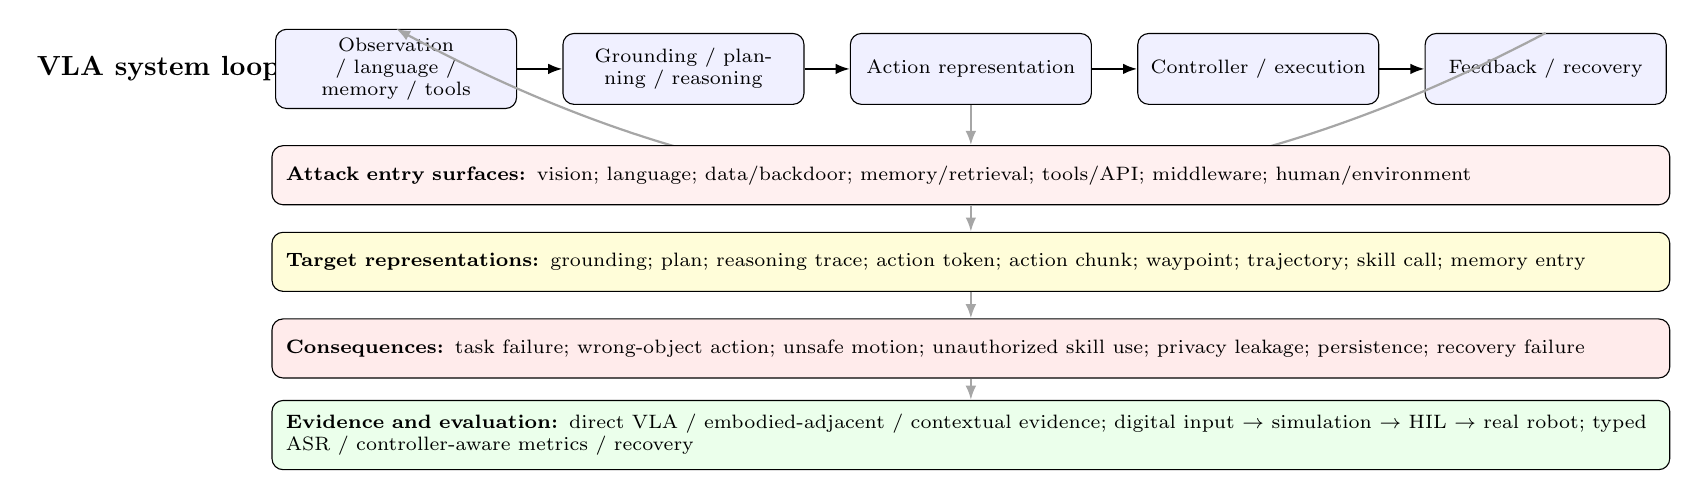
\begin{tikzpicture}[
    font=\scriptsize,
    loop/.style={draw, rounded corners, align=center, text width=2.85cm, minimum height=0.9cm, inner sep=3pt, fill=blue!6},
    band/.style={draw, rounded corners, align=left, text width=17.4cm, minimum height=0.75cm, inner sep=5pt},
    arr/.style={-{Latex[length=1.8mm]}, thick},
    softarr/.style={-{Latex[length=1.8mm]}, thick, gray!70}
]
\node[anchor=east, font=\bfseries] at (-1.35,0) {VLA system loop};
\node[loop] (obs) at (0,0) {Observation / language / memory / tools};
\node[loop] (reason) at (3.65,0) {Grounding / planning / reasoning};
\node[loop] (action) at (7.3,0) {Action representation};
\node[loop] (ctrl) at (10.95,0) {Controller / execution};
\node[loop] (feed) at (14.6,0) {Feedback / recovery};
\draw[arr] (obs) -- (reason);
\draw[arr] (reason) -- (action);
\draw[arr] (action) -- (ctrl);
\draw[arr] (ctrl) -- (feed);
\draw[arr, gray!70] (feed.north) to[bend left=28] node[above, font=\scriptsize] {future observations and state} (obs.north);

\node[band, fill=red!6] (entry) at (7.3,-1.35) {\textbf{Attack entry surfaces:} vision; language; data/backdoor; memory/retrieval; tools/API; middleware; human/environment};
\node[band, fill=yellow!15] (target) at (7.3,-2.45) {\textbf{Target representations:} grounding; plan; reasoning trace; action token; action chunk; waypoint; trajectory; skill call; memory entry};
\node[band, fill=red!8] (cons) at (7.3,-3.55) {\textbf{Consequences:} task failure; wrong-object action; unsafe motion; unauthorized skill use; privacy leakage; persistence; recovery failure};
\node[band, fill=green!8] (eval) at (7.3,-4.65) {\textbf{Evidence and evaluation:} direct VLA / embodied-adjacent / contextual evidence; digital input $\rightarrow$ simulation $\rightarrow$ HIL $\rightarrow$ real robot; typed ASR / controller-aware metrics / recovery};
\draw[softarr] (action.south) -- (entry.north);
\draw[softarr] (entry.south) -- (target.north);
\draw[softarr] (target.south) -- (cons.north);
\draw[softarr] (cons.south) -- (eval.north);
\end{tikzpicture}
}
\caption{VLA attack survey overview. The figure summarizes the scope of the survey by linking the VLA system loop to attack entry surfaces, target representations, consequences, and evidence/evaluation levels.}
\label{fig:survey-overview}
\end{figure*}

\section{Closed-Loop Propagation of VLA Attacks}
\label{sec:taxonomy}

\subsection{Closed-Loop VLA System}

A VLA-enabled robot should be read as a closed-loop state transition system, not as a single prompt-to-action function. Let $x_t$ denote the physical state, $o_t=O(x_t,\eta_t)$ the observation produced by sensors and preprocessing noise $\eta_t$, $m_t$ the memory/tool/human context, and $u_t$ the command emitted by the VLA or its planner. A low-level controller $K$ maps $u_t$ and robot state to actuation, while a recovery or safety mechanism $R$ may stop, replan, filter, or ask for help:
\begin{align}
    u_t &= \pi_\theta(o_{\le t}, g, m_t), \nonumber\\
    a_t &= K(u_t, x_t, R_t), \nonumber\\
    x_{t+1} &= F(x_t, a_t, w_t), \quad m_{t+1}=U(m_t,o_t,u_t,a_t).
    \label{eq:closed-loop-vla}
\end{align}
The safety envelope is a set $\mathcal{S}$ over physical state, controller state, tool authorization, privacy state, and human proximity. An attack is relevant when an intervention $\delta$ changes one of these transitions or contexts so that the rollout violates a task, authorization, privacy, or safety predicate. This view gives the survey its central question: where does the adversary enter, which representation changes first, how does that change cross the controller boundary, and does feedback or recovery stop it?

Figure~\ref{fig:vla-pipeline} is the organizing framework for the rest of the survey. It separates where the adversary enters from what the attack changes, marks the controller boundary, and summarizes the propagation chain
\begin{align}
\delta &\rightarrow \Delta o_t \rightarrow \Delta z_t
\rightarrow \Delta u_t \rightarrow \Delta a_t \nonumber\\
&\rightarrow \Delta x_{t+1}
\rightarrow \text{recovery or violation}
\label{eq:attack-propagation}
\end{align}
The same perturbation can stop at the observation, change an embedding or grounding representation, alter a plan, shift an action token, corrupt a chunk, redirect a trajectory, be clipped by a controller, or only become visible after the next observation. This is why a VLA attack claim is not settled at the model-output boundary; the robot-level claim depends on execution, feedback, recovery, and the resulting physical or system consequence.

\subsection{Attack Map}

The attack map has four intuitive stages. First, the attack enters through a channel: vision, language, memory, tool output, middleware, training data, physical environment, or human interaction. Second, it changes a target representation: grounding, plan, reasoning trace, action token, action chunk, waypoint, trajectory, velocity field, controller state, memory entry, or tool call. Third, the changed representation reaches a robot or system consequence: task failure, wrong-object action, unsafe motion, unauthorized skill use, privacy leakage, or persistent state compromise. Fourth, the validation setting determines what the claim can support: digital input, real-sensor input, simulation rollout, hardware-in-the-loop, real-robot actuation, or human-proximate study.

Table~\ref{tab:taxonomy-overview} keeps these stages orthogonal because common labels hide different mechanisms. ``Physical attack'' describes an access channel, not the target: a physical patch may attack visual embeddings, grounding, visual proprioception, or a trajectory objective. ``Jailbreak'' describes a family resemblance, not a consequence: a prompt attack may cause task failure, targeted motion, unauthorized tool use, or no robot-level effect. ``Backdoor'' describes timing and training access, but the robotic target may be a gripper primitive, an action chunk, a waypoint, or a long-horizon trajectory.

\begin{table*}[t]
\centering
\footnotesize
\caption{Orthogonal multi-axis taxonomy for coding VLA attacks. Each paper may receive multiple labels on each axis; axes are not mutually exclusive categories.}
\label{tab:taxonomy-overview}
\renewcommand{\arraystretch}{1.08}
\setlength{\tabcolsep}{2.4pt}
\begin{tabularx}{\textwidth}{@{}p{0.16\textwidth}Y Y@{}}
\toprule
\textbf{Axis} & \textbf{Allowed labels} & \textbf{Coding question} \\
\midrule
Lifecycle & Training; inference; runtime; post-deployment & When is the adversarial intervention introduced or activated? \\
Entry surface & Vision; language; state; memory; tool; middleware; human; environment & Which semantic or system channel carries the adversarial content? \\
Target component & Visual encoder; language encoder; multimodal projector; planner/reasoner; action head; controller; memory; tool/API; middleware & Which system component is attacked or measured? \\
Target representation & Embedding; grounding; plan; action token; chunk; waypoint; trajectory; velocity field; controller state; memory entry & Which representation or control object changes inside or across components? \\
Security property violated & Availability; integrity; confidentiality; authorization & Which security property is violated? Physical safety is represented as a consequence rather than merged into this axis. \\
Knowledge level & White-box; gray-box; black-box; transfer-only; unknown & What does the attacker know about weights, gradients, architecture, prompts, action heads, or controllers? \\
Access channel & Digital; physical; human-mediated; supply-chain; hybrid & How does the attacker deliver the intervention? This is separate from knowledge level. \\
Privilege level & User; bystander; operator; data contributor; model provider; tool/API; middleware; no privilege & What role or privilege boundary does the attacker occupy or abuse? \\
Temporal profile & One-shot; repeated; delayed; persistent & Does the attack act once, recur over feedback, activate later, or survive sessions/training? \\
Validation tier & Digital input; real sensor; simulation; HIL; robot actuation; human-proximate & What is the strongest demonstrated validation tier? Do not infer actuation or human proximity from input-only tests. \\
Consequence & Task failure; wrong object; unsafe action; collision/contact risk; privacy leakage; unauthorized skill; persistent state compromise & What happened at the robot/system boundary? Keep consequence separate from objective and entry surface. \\
\bottomrule
\end{tabularx}
\end{table*}


\subsection{Typed Attack Success}
\label{subsec:attack-success}

Because VLA safety papers do not yet use a uniform definition of attack success, a survey needs a typed definition. Let $\tau^0(c)$ be the benign rollout from an initial condition and task context $c=(x_0,g,m_0)$, and let $\tau^\delta(c)$ be the rollout under an adversarial intervention $\delta$ that satisfies the declared knowledge, access, privilege, budget, and physical constraints. A VLA attack is successful for objective type $O$ and consequence class $C$ when
\begin{align}
    \mathrm{Succ}_{O,C}(\tau^\delta,\tau^0)
    &= \mathbf{1}\{ \phi_{O,C}(\tau^\delta)=1 \nonumber\\
    &\quad \land\ \phi_{O,C}(\tau^0)=0
    \land\ \delta \in \Delta(\mathcal{A}) \}.
    \label{eq:attack-success}
\end{align}
where $\phi_{O,C}$ is a typed violation predicate and $\Delta(\mathcal{A})$ is the admissible attacker set. The benign rollout condition prevents ordinary task difficulty or non-adversarial distribution shift from being counted as attack success. If a benign rollout is unavailable, the paper should state the baseline used, such as clean task success, human-labeled intended behavior, or non-member trajectory statistics.

The predicate $\phi_{O,C}$ must be typed. A \emph{task-failure attack} succeeds when the benign task would complete but the attacked rollout fails. A \emph{targeted behavior attack} succeeds when the robot reaches an attacker-specified object, action primitive, waypoint, trajectory, skill, or tool call. A \emph{safety attack} succeeds when the rollout violates a safety envelope, contact margin, force/velocity/workspace bound, or human-proximity constraint. An \emph{authorization attack} succeeds when the system executes an unauthorized command, skill, tool, or privilege transition. A \emph{privacy attack} succeeds when membership, trajectory, user, or scene information is inferred above a stated threshold. A \emph{persistence attack} succeeds when the adversarial effect survives replanning, feedback, memory update, fine-tuning, or a session boundary. A \emph{recovery-failure attack} succeeds when the system has an opportunity to stop, replan, ask for help, or invoke a recovery policy but still reaches the violation predicate.

This definition makes ASR meaningful only when five items are stated together: the violation predicate, the denominator, the attacker assumptions, the validation tier, and the benign or clean baseline. Without these items, ASR values from different VLA papers should be treated as local evidence rather than comparable field-level rates.

\begin{figure*}[t]
\centering
\scriptsize
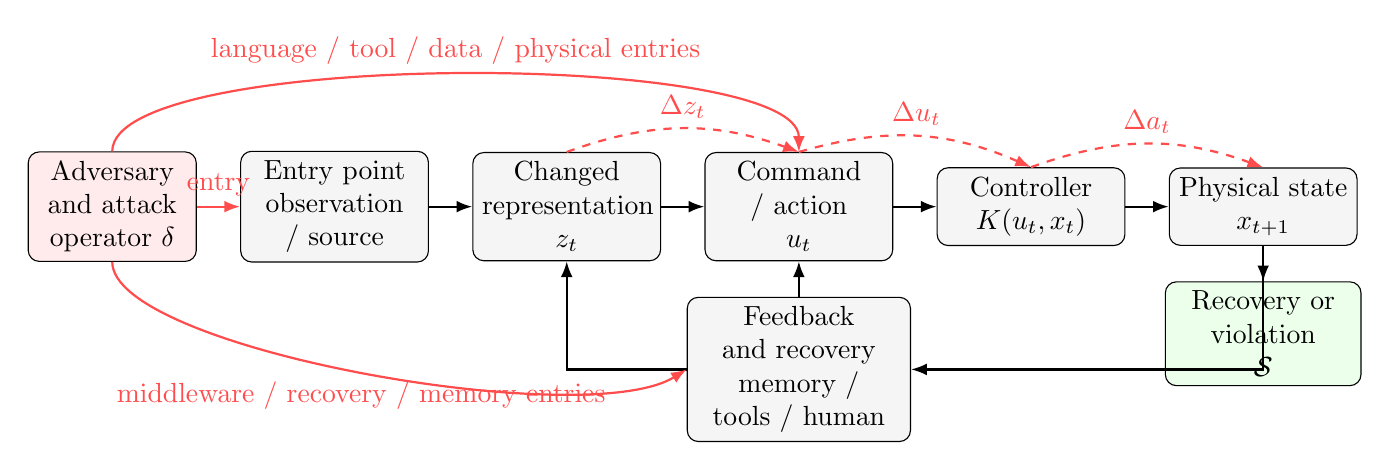
\begin{tikzpicture}[
    node distance=0.45cm and 0.55cm,
    box/.style={draw, rounded corners, align=center, minimum height=0.95cm, text width=2.15cm, fill=gray!8},
    atk/.style={draw, rounded corners, align=center, text width=2.2cm, fill=red!8},
    arr/.style={-{Latex[length=2mm]}, thick}
]
\node[box] (obs) {Entry point\\observation / source};
\node[atk, left=of obs, text width=1.9cm] (adv) {Adversary\\and attack\\operator $\delta$};
\node[box, right=of obs] (latent) {Changed\\representation\\$z_t$};
\node[box, right=of latent] (cmd) {Command / action\\$u_t$};
\node[box, right=of cmd] (ctrl) {Controller\\$K(u_t,x_t)$};
\node[box, right=of ctrl] (exec) {Physical state\\$x_{t+1}$};
\node[box, below=of cmd, text width=2.6cm] (rec) {Feedback and recovery\\memory / tools / human};
\node[box, below=of exec, text width=2.25cm, fill=green!8] (safe) {Recovery or\\violation\\$\mathcal{S}$};
\draw[arr] (obs) -- (latent);
\draw[arr] (latent) -- (cmd);
\draw[arr] (cmd) -- (ctrl);
\draw[arr] (ctrl) -- (exec);
\draw[arr] (exec.south) -- (safe.north);
\draw[arr] (exec.south) |- (rec.east);
\draw[arr] (rec.west) -| (latent.south);
\draw[arr] (rec.north) -- (cmd.south);
\draw[arr, red!70] (adv) -- node[above, sloped] {entry} (obs);
\draw[arr, red!70] (adv.north) .. controls +(0,1.3) and +(0,1.3) .. node[above] {language / tool / data / physical entries} (cmd.north);
\draw[arr, red!70] (adv.south) .. controls +(0,-1.1) and +(-1.3,-0.8) .. node[below] {middleware / recovery / memory entries} (rec.west);
\draw[arr, red!70, dashed] (latent.north) to[bend left=20] node[above] {$\Delta z_t$} (cmd.north);
\draw[arr, red!70, dashed] (cmd.north) to[bend left=20] node[above] {$\Delta u_t$} (ctrl.north);
\draw[arr, red!70, dashed] (ctrl.north) to[bend left=20] node[above] {$\Delta a_t$} (exec.north);
\end{tikzpicture}
\caption{Core closed-loop view used throughout the survey. The figure separates adversarial entry surfaces from representation impact, marks the controller boundary between model command and physical actuation, and shows how feedback either supports recovery or carries the system toward a robot/system violation.}
\label{fig:vla-pipeline}
\end{figure*}

\subsection{Attacker Assumptions}

We assume the deployer has an intended task, authorized users, authorized tools and skills, and a safety envelope for people, property, data, and robot hardware. The attacker seeks to violate one or more of these constraints while preserving enough surface plausibility that the system continues acting, logs the event as normal, or stores corrupted context for future sessions.

Attacker capability has three independent dimensions. \emph{Knowledge level} describes what the attacker knows about weights, gradients, architecture, prompts, action heads, or controllers: white-box, gray-box, black-box, transfer-only, or unknown. \emph{Access channel} describes how the intervention is delivered: digital, physical, human-mediated, supply-chain, or hybrid. \emph{Privilege level} describes the role or boundary involved: user, bystander, operator, data contributor, model provider, tool/API, middleware, or no privilege. Keeping these dimensions separate prevents a common confusion: ``black-box'' and ``physical'' are not alternatives. A physical patch can be optimized with white-box gradients, transferred in a black-box setting, or deployed by a bystander with no digital privileges.

\subsection{Reading the Map Through Examples}

The map is easiest to read through examples. In a scene-text hijacking scenario, the attacker does not need to rewrite the user's goal; the robot sees an instruction-like phrase in the environment, the phrase changes source grounding or plan selection, and the downstream consequence may be wrong-object manipulation or unauthorized skill use. In a patch scenario, the entry is visual, but the relevant question is whether the perturbation merely changes an embedding or whether it reaches an action token, waypoint, or physical trajectory \cite{wang2025vlaadversarial,xu2025edpa,lu2026patch}. In a poisoned-demonstration scenario, the attack enters before deployment, hides behind clean utility, and later activates as a gripper primitive, action freeze, or chunk-level drift \cite{wang2025freezevla,xu2025dropvla,xu2026silentdrift}. In a trajectory-redirection scenario, the language may remain close to the user's instruction while the physical path bends toward a different endpoint \cite{puthumanaillam2026trajectory}. In a membership-inference scenario, the consequence is not motion failure at all; action likelihoods or temporal action traces leak whether a demonstration or trajectory was in the training set \cite{peng2026miavla,luan2026vlaleaks}.

This separation also prevents overclaiming. A VLM jailbreak with no robot action is contextual evidence for source confusion, not direct evidence of VLA unsafe action. A ROS2 middleware exploit is embodied-adjacent evidence for tool/middleware compromise, not a VLA policy attack unless the VLA system consumes or emits the compromised message. A physical LiDAR or camera attack can be strong sensor evidence but remains contextual for VLA action unless a VLA-controlled robot rollout is measured.

\section{Evidence Synthesis}
\label{sec:evidence-synthesis}

This section synthesizes the Core Evidence Corpus defined in Section~\ref{sec:methodology}, using contextual references only to interpret mechanisms and substrates. The main pattern is clear: direct VLA attack evidence is now substantial enough to review, but it remains concentrated in OpenVLA/LIBERO-style manipulation, often preprint-heavy, and uneven in physical validation. Embodied-adjacent attacks remain useful for threat modeling, while contextual references should not be written as if they were validated VLA attacks.

\begin{table*}[t]
\centering
\scriptsize
\caption{Evidence-aware synthesis by corpus. Core rows are attack evidence; contextual rows support taxonomy or evaluation but are not included in attack-study denominators. D: digital; S: simulation; HIL: hardware-in-the-loop; P: physical robot/world; PR: peer-reviewed; PP: preprint or non-archival version.}
\label{tab:attack-literature-summary}
\renewcommand{\arraystretch}{1.1}
\setlength{\tabcolsep}{1.8pt}
\begin{tabularx}{\textwidth}{@{}p{0.13\textwidth}p{0.28\textwidth}p{0.10\textwidth}p{0.11\textwidth}Y@{}}
\toprule
\textbf{Corpus / stratum} & \textbf{Representative work} & \textbf{Status} & \textbf{Validation} & \textbf{What the evidence supports} \\
\midrule
Direct VLA: instruction/control & RoboGCG, VLA-Fool, SABER, Q-DIG, trajectory redirection \cite{jones2025robogcg,yan2025vlafool,wu2026saber,srikanth2026qdig,puthumanaillam2026trajectory} & PP & D/S/P & Language or multimodal perturbations can alter VLA rollout behavior; black-box, natural-prompt, and command-preserving settings are emerging. \\
Direct VLA: patches/physical vision & ICCV patch attacks, EDPA, ADVLA, UPA-RFAS, VLA-Hijack, Tex3D, partially observable patches \cite{wang2025vlaadversarial,xu2025edpa,zhang2025advla,lu2026patch,fu2026vlahijack,chen2026tex3d,wang2026partialpatch} & PR/PP & D/S/P & Visual attacks can target embeddings, grounding, visual proprioception, action trajectories, and object textures; transfer and physical evidence are improving but uneven. \\
Direct VLA: action/backdoor & FreezeVLA, BadVLA, GoBA, DropVLA/TabVLA, AttackVLA/BackdoorVLA, SilentDrift \cite{wang2025freezevla,zhou2025badvla,zhou2025goba,xu2025dropvla,li2025attackvla,xu2026silentdrift} & PP & S/P & VLA attacks can target action primitives, action freezing, chunk drift, and long-horizon triggered behavior, often while preserving clean utility. \\
Direct VLA: reasoning/privacy & TRAP, altered reasoning traces, ReasonBreak, VLA membership inference, VLALeaks \cite{huang2026trap,altered2026thoughts,teymoorianfard2026reasonbreak,peng2026miavla,luan2026vlaleaks} & PP & D/S/P & Reasoning traces and training membership are VLA-specific target representations; objectives include integrity and confidentiality rather than only task failure. \\
Core: embodied-adjacent attacks & BadRobot, RoboPAIR, CHAI, RoboJailBench, ANNIE, Phantom Menace, Eva-VLA \cite{zhang2025badrobot,robey2025robopair,burbano2025chai,yeke2026robojailbench,huang2025annie,lu2025phantom,liu2025evavla} & PR/PP & D/S/P & Embodied LLM/VLM, environmental command, trajectory, sensor, and physical-variation attacks inform VLA threat models but are not counted as direct VLA evidence unless VLA policies are attacked. \\
Contextual references & VLA/RFM substrates, benchmarks, adversarial ML, physical/sensor attacks, RAG/tool-agent security, RL backdoors, ROS/robot cybersecurity \cite{kim24openvla,black2024pi0,liu2023libero,goodfellow2015explaining,brown2017adversarial,cao2019lidar,zou2025poisonedrag,debenedetti2024agentdojo,kiourti2020trojdrl,deng2022insecurityros2} & PR/PP & D/S/P & Provides mechanisms, substrates, and evaluation lessons; not included in attack-study denominators unless the work has explicit attacker, target, method, and outcome. \\
\bottomrule
\end{tabularx}
\end{table*}


\subsection{Training-Time and Supply-Chain Attacks}

\textbf{Direct evidence.} VLA backdoor work has expanded from generic task disruption to action and trajectory control. BadVLA studies objective-decoupled VLA backdoors that preserve clean performance while inducing triggered action deviations \cite{zhou2025badvla}. Its evidence is direct because the victim is a VLA policy and the measured output is action behavior, but its strongest claims are still tied to the particular trigger, benchmark, and fine-tuning setup. GoBA changes the threat model by using ordinary physical objects as goal-oriented triggers and by introducing BadLIBERO-style evaluation with ``nothing to do,'' ``try to do,'' and ``success to do'' levels \cite{zhou2025goba}. This is stronger than a binary failure label because it distinguishes a triggered attempt from completed attacker-specified behavior.

DropVLA/TabVLA narrows the target further to reusable low-level action primitives, such as gripper release, under small poisoning budgets and reports simulation plus physical feasibility \cite{xu2025dropvla}. Its main contribution for a robotics audience is temporal precision: the attack is not only that a task fails, but that a primitive fires at a decision window. AttackVLA then provides a broader evaluation harness for adversarial and backdoor attacks and introduces BackdoorVLA for attacker-specified long-horizon action sequences \cite{li2025attackvla}. SilentDrift is especially robotics-relevant because it attacks action chunking and delta-pose integration, showing how small poisoned drifts can accumulate during intra-chunk open-loop execution \cite{xu2026silentdrift}. Together, these papers show a progression from \emph{triggered failure} to \emph{triggered goal behavior}, \emph{primitive-level control}, and \emph{chunk-level trajectory drift}. They should not be collapsed into one backdoor category.

\textbf{Evidence strength and gaps.} The direct VLA backdoor evidence is stronger than analogies from classifiers because it measures action traces and clean-task retention. It is still not yet field-wide evidence. Most studies use curated manipulation suites and controlled triggers; few report how data inspection, trajectory validation, controller clipping, or post-training updates affect attack survival. Few compare whether the same trigger works across autoregressive token heads, continuous action heads, action chunks, and flow/diffusion policies. These gaps matter because training-time attacks become deployment risks only if the trigger persists through the actual adaptation pipeline, robot morphology, camera placement, and controller.

\textbf{Embodied-adjacent and analogical evidence.} Classic poisoning and backdoor attacks establish the general supply-chain risk \cite{biggio2012poisoning,gu2017badnets,liu2018trojaning,carlini2024poisoningweb}, and RL backdoors show that sequential policies can learn trigger-conditioned behavior \cite{kiourti2020trojdrl,wang2021backdoorl,cui2024badrl,rathbun2025inception}. These works justify VLA backdoor threat models but do not by themselves prove VLA vulnerability. The direct VLA backdoor papers now provide that evidence, with the caveat that most remain recent preprints and frequently rely on a small set of benchmarks and robot embodiments.

\subsection{Perception, Multimodal, and Physical Attacks}

\textbf{Direct evidence.} Early VLA patch work formulates action-discrepancy, position-aware, and targeted manipulation objectives and evaluates digital plus physical patch settings \cite{wang2025vlaadversarial}. This work is important because the objective is defined in action space rather than as image classification error. VLA-Fool expands the attack surface to textual, visual, and cross-modal misalignment attacks under white-box and black-box settings \cite{yan2025vlafool}. Its strongest value is not a single failure number, but the comparison across language perturbations, visual patches/noise, and image--instruction mismatch.

EDPA reduces the required attacker knowledge by targeting visual encoder embeddings and cross-modal alignment rather than the full action head \cite{xu2025edpa}. ADVLA pushes a related gray-box direction by using attention-guided sparse feature-space perturbations that are low-amplitude and patch-wise localized \cite{zhang2025advla}. Universal transferable patch work, such as UPA-RFAS, studies black-box transfer across VLA models, prompts, viewpoints, and sim-to-real settings \cite{lu2026patch}. VLA-Hijack targets visual proprioception by suppressing real-arm features and injecting a phantom embodiment patch, exposing a representation-level reason for cross-architecture transfer \cite{fu2026vlahijack}. Tex3D moves from 2D patches to adversarial object textures optimized over long-horizon trajectories and evaluated in simulation and real-robot settings \cite{chen2026tex3d}. Partially observable patch attacks further constrain the adversary to a short trajectory prefix, a more realistic physical-access setting \cite{wang2026partialpatch}.

These papers form a useful sequence of evidence. Action-space patches ask whether visual perturbations can change robot motion. Embedding and attention attacks ask whether attacking the shared VLM/VLA representation is enough when the action head is unknown. Transferable patches ask whether the attack survives architecture, fine-tuning, and viewpoint changes. 3D texture attacks ask whether the attack can be bound to manipulated objects rather than pasted into the camera frame. Partial-observation attacks ask whether the adversary can attack without seeing the full future rollout. The sequence is more informative than a single ``visual attack'' bucket.

\textbf{Analogical evidence.} Foundational adversarial examples, physical patches, object-detector attacks, 3D mesh attacks, LiDAR attacks, and audio-command attacks show that physical sensor inputs can be manipulated \cite{szegedy2014intriguing,goodfellow2015explaining,papernot2016limitations,carlini2017towards,kurakin2017physical,brown2017adversarial,moosavi2017universal,madry2018towards,athalye2018synthesizing,eykholt2018robust,eykholt2018detectors,chen2018shapeshifter,thys2019fooling,xu2020tshirt,xiao2019meshadv,cao2019lidar,tu2020lidar,sun2020robustlidar,cao2021invisible,carlini2016hiddenvoice,zhang2017dolphinattack,yuan2018commandersong,sugawara2020lightcommands}. Their direct implication for VLA systems depends on whether the perturbation changes grounding, plan, action, trajectory, or recovery. This is why VLA patch papers should report action traces and consequence labels rather than only image-level success.

\subsection{Instruction, Planning, and Reasoning Attacks}

\textbf{Direct evidence.} RoboGCG adapts adversarial prompt optimization to VLA control authority and shows that a prompt-level intervention at rollout start can influence action reachability over time \cite{jones2025robogcg}. Its claim is stronger than a text jailbreak claim because the target is robot action reachability, but the access and optimization assumptions still need to be reported whenever the result is cited. SABER makes the instruction threat model more practical by using a black-box, agentic edit process with bounded character/token/prompt edits and rollout-level feedback across multiple VLA models \cite{wu2026saber}. Q-DIG approaches red-teaming differently: rather than optimizing a single adversarial suffix, it uses quality-diversity search to generate natural, task-relevant instructions that expose robot-policy failures and can be used for robustness improvement \cite{srikanth2026qdig}. Trajectory-level redirection studies command-preserving prompts that keep the instruction close to the intended task while redirecting the physical outcome \cite{puthumanaillam2026trajectory}.

Reasoning-enabled VLAs create an additional internal target. TRAP shows that CoT or intermediate reasoning traces can be hijacked by physical patches to steer downstream actions without changing the user's instruction \cite{huang2026trap}. Altered-thought studies further indicate that entity references in VLA reasoning traces can causally affect robot manipulation success, while non-reasoning control models may be immune to that specific channel \cite{altered2026thoughts}. ReasonBreak extends the reasoning-trajectory question to autonomous-driving-style VLA systems and evaluates black-box textual corruptions against reasoning and trajectory safety metrics in closed-loop simulation \cite{teymoorianfard2026reasonbreak}. The shared lesson is that reasoning text is neither merely explanation nor merely prompt context; in some VLA designs it is a control-relevant representation.

\textbf{Embodied-adjacent evidence.} BadRobot, RoboPAIR, CHAI, SafeAgentBench, EARBench, and RoboJailBench evaluate embodied jailbreak, physical command hijacking, and risk-aware planning where success is measured closer to action than text-only refusal \cite{zhang2025badrobot,robey2025robopair,burbano2025chai,yin2024safeagentbench,zhu2024earbench,yeke2026robojailbench}. These are important for goal hijacking and HRI threat models, but they should be labeled as embodied-adjacent when the target is not a VLA policy.

\subsection{Action-Level and Closed-Loop Attacks}

Action representation is the robotics core of this review. Autoregressive action-token policies expose token probabilities and discretized gripper/pose bins; a prompt or patch can change which token is selected, and early token errors can propagate through subsequent actions. RT-1, RT-2, OpenVLA, and SpatialVLA illustrate tokenized or discretized action interfaces whose action vocabulary, spatial grids, or detokenizers become attack-relevant representations \cite{brohan2022rt1,brohan2023rt2,kim24openvla,qu2025spatialvla}. Parallel action chunks create a different risk: the model commits to several future actions before new observations can correct the error. ACT, OpenVLA-OFT, and related high-throughput VLA fine-tuning recipes show why chunk length, temporal ensemble, and parallel decoding should be reported as security variables rather than only efficiency variables \cite{zhao2023act,kim2025openvlaoft}. SilentDrift directly exploits this intra-chunk open-loop property \cite{xu2026silentdrift}.

Waypoint and trajectory policies expose geometric objectives such as end-effector displacement, curvature, unsafe workspace entry, or targeted path redirection \cite{wang2025vlaadversarial,puthumanaillam2026trajectory}. Planner-mediated systems such as CLIPort, Code as Policies, ProgPrompt, and VoxPoser make object binding, generated code, value maps, and waypoint fields explicit enough to inspect but also explicit enough to attack \cite{shridhar2022cliport,liang2023code,singh2023progprompt,huang2023voxposer}. Diffusion and flow policies, including Diffusion Policy and $\pi_0$, shift the target from a token to a conditional trajectory distribution, denoising path, velocity field, or sampling process \cite{chi2023diffusion,black2024pi0}. Generalist policy and dataset work such as Octo, Open X-Embodiment, DROID, BridgeData, RoboNet, and Gato further matter because they define the cross-embodiment and data-provenance assumptions under which attacks may or may not transfer \cite{ghosh2024octo,openx2023,khazatsky2024droid,walke2023bridgedata,dasari2019robonet,reed2022gato}.

The closed-loop consequence depends on controller and recovery design. A temporal ensemble can damp high-frequency perturbations but may also prolong a poisoned action chunk. A high re-planning frequency can recover from one-frame perception attacks but may be vulnerable to repeated low-amplitude nudges. Controller latency and stale observations can turn a semantically correct command into an unsafe physical action. Safety envelopes and low-level controllers can prevent direct collision while still allowing wrong-object manipulation, unauthorized skill use, privacy leakage, or near-boundary behavior. Therefore, direct VLA attack papers should report not only ASR but also first affected representation, action deviation, recovery opportunity, controller intervention, and whether the safety envelope changed the outcome.

\subsection{System, Memory, Tool, HRI, and Persistent Attacks}

\textbf{Embodied-adjacent evidence.} Tool-agent attacks and indirect prompt injection show how untrusted context can override source boundaries and cause tool misuse or data leakage \cite{greshake2023not,yi2023bipia,zhan2024injecagent,ruan2024toolemu,debenedetti2024agentdojo}. In robotics, the analogous failure can become an unauthorized skill call, unsafe tool argument, or middleware command, but most evidence remains adjacent rather than directly VLA-validated. Toolformer, ReAct, Gorilla, ToolLLM, WebShop, and WebArena are useful here only as software-agent substrates; they should not be counted as VLA evidence unless robot skills or VLA-controlled actions are in the loop \cite{schick2023toolformer,yao2023react,patil2023gorilla,qin2023toolllm,yao2022webshop,zhou2023webarena}. ROS/ROS2 and robot cybersecurity work show that middleware, topics, services, node identity, and controller interfaces can be compromised \cite{quigley2009ros,dieber2020penetration,deng2022insecurityros2,quarta2017industrial,bonaci2015surgical,mayoral2020robot,yaacoub2022robotics,neupane2024security}. HRI work shows that robots can affect human trust, authority, and physical access decisions \cite{booth2017piggybacking,postnikoff2018robot,bainbridge2011benefits,saunderson2021persuasive}.

\textbf{Analogical evidence.} RAG and memory poisoning show how retrieved context can be corrupted and later reused \cite{zhong2023poisoning,deng2024pandora,zou2025poisonedrag,cho2024garag}. For VLA systems, the unvalidated but important hypothesis is multi-session embodied memory compromise: a poisoned object memory, map, user preference, or tool log could redirect future robot behavior. This remains mostly an open VLA attack problem, not a demonstrated field-wide result.

\section{Cross-Study Comparison and Evidence Gaps}
\label{sec:cross-study}

This section distills what the current evidence says across attack mechanisms. We use the core attack studies as the denominator for cross-study claims and use contextual references only to explain substrates and evaluation concepts. The key point is that attacks should be compared by mechanism, validation tier, action representation, and consequence, not by a single undifferentiated ASR.

\begin{table*}[t]
\centering
\scriptsize
\caption{Descriptive statistics from frozen database \texttt{VLA-Attack-ER-v2026-06-16}. Attack-study statistics use the Core Evidence Corpus unless a direct-VLA subset is explicitly named; NR is counted as not reported.}
\label{tab:evidence-statistics}
\renewcommand{\arraystretch}{1.08}
\setlength{\tabcolsep}{3pt}
\begin{tabularx}{\textwidth}{@{}p{0.22\textwidth}Y@{}}
\toprule
\textbf{Statistic} & \textbf{Observed pattern} \\
\midrule
Corpus split & 85 records: 30 core attack studies (23 direct VLA and 7 embodied-adjacent) plus 55 contextual references. \\
Direct VLA subset & 23/30 core attack studies are direct VLA evidence; all percentages below use the direct subset ($n=23$). \\
Entry surface flags in direct VLA & Visual/physical visual input: 14/23 (60.9\%); language/instruction: 9/23 (39.1\%); reasoning-trace input: 1/23 (4.3\%); privacy/query output: 2/23 (8.7\%); poisoned trajectory/data trigger: 1/23 (4.3\%). Multi-label counts overlap. \\
Knowledge level & Any black-box or transfer-only condition: 13/23 (56.5\%); any white/gray-box optimization condition: 14/23 (60.9\%). Multi-label counts overlap when papers report multiple settings. \\
Access and privilege & Digital access channel: 14/23 (60.9\%); physical or digital-to-physical channel: 8/23 (34.8\%); supply-chain or data-contributor channel: 5/23 (21.7\%). \\
Highest validation tier & Digital input-only: 3/23 (13.0\%); simulation rollout: 10/23 (43.5\%); real-sensor input: 1/23 (4.3\%); real-robot actuation: 9/23 (39.1\%); HIL: 0/23 (0\%); human-proximate: 0/23 (0\%). \\
Model/benchmark concentration & OpenVLA-family target appears in 10/23 (43.5\%); LIBERO appears in 12/23 (52.2\%); $\pi_0/\pi_0$-fast appears in 6/23 (26.1\%). \\
Reporting practices & Explicit transfer beyond one target/model/prompt: 16/23 (69.6\%); limited transfer notes: 6/23 (26.1\%); benign utility reported: 7/23 (30.4\%); query/edit budget reported: 6/23 (26.1\%). \\
Robot-control reporting & Action/chunk horizon reported: 3/23 (13.0\%); controller frequency reported: 1/23 (4.3\%); safety filter reported: 0/23 (0\%); recovery policy/outcome reported: 0/23 (0\%); pre/post-controller trace: 0/23 (0\%). \\
\bottomrule
\end{tabularx}
\end{table*}


\begin{table*}[t]
\centering
\scriptsize
\caption{Representative direct VLA attack mechanisms and what each mechanism currently supports. The table is qualitative: it summarizes mechanism-level evidence rather than pooling heterogeneous ASR values.}
\label{tab:core-heatmaps}
\renewcommand{\arraystretch}{1.08}
\setlength{\tabcolsep}{3pt}
\begin{tabularx}{\textwidth}{@{}p{0.17\textwidth}Y Y Y Y@{}}
\toprule
\textbf{Attack family} & \textbf{Representative entry} & \textbf{Changed representation} & \textbf{Robotic consequence} & \textbf{Evidence strength and caveat} \\
\midrule
Instruction/control & Prompt edit, scene text, or cross-modal instruction perturbation & Plan, source grounding, action token, or command-preserving trajectory & Task failure, action inflation, wrong-object behavior, or trajectory redirection & Direct rollout evidence is emerging; transfer, query budget, and recovery still vary across studies. \\
Visual/physical & Digital patch, printed patch, object texture, or partial-observation physical access & Embedding, grounding, visual proprioception, action loss, or trajectory objective & Wrong-object action, targeted motion, trajectory deviation, or degraded manipulation & Strong mechanism evidence across digital, simulation, and some real-robot settings; physical generality across viewpoints, objects, and controllers remains open. \\
Backdoor/action & Poisoned demonstration, trigger object, or supply-chain fine-tuning & Primitive, action freeze, chunk drift, waypoint, or long-horizon action sequence & Triggered release/freeze, wrong goal behavior, or gradual trajectory shift & Direct VLA studies show action representations are attackable while preserving clean utility; robustness to filtering, adaptation, and controller clipping is less mature. \\
Reasoning/privacy & Physical/contextual reasoning perturbation or action-trace query access & CoT/entity reference, reasoning-to-action state, likelihood, attention, or temporal trajectory signature & Reasoning hijack, unsafe driving/manipulation behavior, or training-membership leakage & Expands the field beyond task-failure ASR; privacy and reasoning claims require metrics different from physical task success. \\
\bottomrule
\end{tabularx}
\end{table*}


\subsection{What Current Evidence Tells Us}

The first lesson is that VLA attacks are increasingly \emph{representation attacks}, not only input perturbations. Visual patches matter because they can move embeddings, grounding, visual proprioception, and trajectory objectives; instruction attacks matter because text can steer plans and action tokens; backdoors matter because triggers can bind to reusable action primitives or chunks. This explains why a survey organized only by input modality misses the robotics mechanism.

The second lesson is that closed-loop evidence is still thin. Many papers show that an attack changes a rollout, but fewer show what happens between the VLA output and the physical state: controller clipping, safety filtering, latency, emergency stop, or recovery. Current evidence therefore supports claims about vulnerable VLA representations more strongly than claims about deployed robot hazard rates.

The third lesson is that the field is splitting into two complementary directions. One direction seeks stronger and more realistic attackers: black-box instruction edits, transferable patches, object-bound 3D textures, partial-observation attacks, and supply-chain triggers. The other direction seeks better evaluation: typed ASR, clean utility, transfer axes, validation tiers, and privacy metrics. A mature VLA attack literature will need both; stronger attacks without robotics-aware evaluation will not answer T-RO-relevant safety questions, and evaluation protocols without adaptive attacks will underestimate residual risk.

\subsection{Direct VLA Evidence by Attack Mechanism}

The direct matrix separates four mechanism families that are often conflated. First, instruction-control attacks operate through language while measuring robot behavior: RoboGCG asks whether adversarial text can give low-level control authority \cite{jones2025robogcg}; SABER asks whether bounded black-box edits can induce task failure, action inflation, or constraint violations across VLA policies \cite{wu2026saber}; Q-DIG asks whether natural, task-relevant prompt diversity can systematically expose VLA policy failures \cite{srikanth2026qdig}; and trajectory redirection asks whether a command-preserving prompt can move the full rollout toward an attacker-specified physical outcome \cite{puthumanaillam2026trajectory}. These are all language-entry attacks, but they differ in objective, attacker cost, and whether the attack is targeted.

Second, visual attacks split into action-loss, representation-loss, transfer, and physical-object variants. Wang et al. optimize VLA-specific action discrepancy and trajectory objectives \cite{wang2025vlaadversarial}. EDPA and ADVLA move the target earlier, toward visual embeddings, projected features, attention, and vision--language alignment \cite{xu2025edpa,zhang2025advla}. UPA-RFAS and VLA-Hijack study transfer by exploiting shared feature-space, attention, semantic, or visual-proprioception structure rather than only a model-specific action head \cite{lu2026patch,fu2026vlahijack}. Tex3D and partially observable patch attacks add physical realism dimensions: object-bound textures, trajectory-aware optimization, and prefix-limited attacker observation \cite{chen2026tex3d,wang2026partialpatch}.

Third, action/backdoor attacks are not merely training-time versions of patches. BadVLA targets trigger-conditioned action deviation \cite{zhou2025badvla}; GoBA targets physical-object-triggered goal behavior \cite{zhou2025goba}; DropVLA targets a reusable primitive at a short reaction window \cite{xu2025dropvla}; AttackVLA compares multiple attack implementations and introduces long-horizon triggered action sequences \cite{li2025attackvla}; FreezeVLA and SilentDrift target action freezing and chunk-level drift \cite{wang2025freezevla,xu2026silentdrift}. The important comparison variable is the attacked action representation: action token, gripper primitive, static action state, full trajectory, or chunked delta-pose sequence.

Fourth, reasoning and privacy attacks expand the objective set. TRAP and altered-thought evaluations show that reasoning traces, entity references, and CoT-to-action pathways can be attack targets in reasoning-enabled VLA systems \cite{huang2026trap,altered2026thoughts}. ReasonBreak shows a related reasoning--trajectory vulnerability in autonomous-driving VLA systems, where closed-loop collision and safety metrics matter more than tabletop task success \cite{teymoorianfard2026reasonbreak}. Membership inference and VLALeaks show that action likelihoods, action errors, temporal motion patterns, attention discrepancies, and trajectory structure can leak training membership \cite{peng2026miavla,luan2026vlaleaks}. These attacks should be evaluated with confidentiality metrics, not forced into task-failure ASR.

\subsection{What Can and Cannot Be Compared}

ASR is not directly comparable across the current VLA attack literature. In one paper, ASR may mean task failure under a visual patch; in another, targeted gripper release within a reaction window; in another, action inflation; in another, trajectory redirection; and in privacy work, AUC or TPR@FPR for membership inference. The denominator also varies: image frames, task episodes, triggered episodes, candidate trajectories, model queries, or physical trials. Validation tier varies from digital input-only to simulation rollout to real-robot actuation. Pooling these numbers would create false precision.

Comparable claims are therefore qualitative and typed. Direct evidence supports the claim that VLA policies can be attacked through vision, language, action representations, backdoors, reasoning traces, and privacy channels. It does not yet support a universal claim that any particular attack transfers across all VLA architectures, embodiments, controllers, or safety envelopes. Embodied-adjacent evidence supports risk hypotheses about source confusion, tool misuse, middleware compromise, sensor corruption, and HRI authority ambiguity. Analogical evidence supports mechanisms and evaluation requirements, not VLA vulnerability claims by itself.

\subsection{Evidence Gaps}

The strongest direct evidence is concentrated in OpenVLA and LIBERO-style manipulation. This is useful because it creates a common baseline, but it weakens claims about general VLA security. Flow/diffusion policies, bimanual systems, mobile manipulation, navigation, tactile policies, and high-level tool/skill interfaces are less consistently covered. Action representations are also unevenly studied: tokenized action heads and patch-induced trajectory deviation are common; diffusion/flow denoising paths, velocity fields, controller latency, temporal ensembling, recovery policies, and safety-envelope interactions are much less mature.

Physical validation is improving but remains narrow. Some direct VLA papers include physical robot demonstrations, but few provide enough detail on sensor stack, control frequency, calibration, lighting, object mass, latency, recovery behavior, and safety filters to make deployment claims portable. Hardware-in-the-loop is surprisingly underdeveloped as a middle tier between simulation and full physical trials.

Privacy is an emerging direct VLA attack area rather than a side issue. Membership inference papers show that VLA training data can leak through action outputs, likelihoods, attention patterns, and temporal motion signatures \cite{peng2026miavla,luan2026vlaleaks}. This evidence is direct, but it supports confidentiality conclusions, not physical-safety conclusions. Future survey tables should therefore include privacy objectives rather than treating all VLA attacks as task-failure attacks.

\subsection{Target Model and Benchmark Concentration}

The target-model distribution is informative evidence. OpenVLA and OpenVLA-OFT appear frequently because they are open, strong, and easy to evaluate on LIBERO \cite{kim24openvla,kim2025openvlaoft,liu2023libero}. $\pi_0$ and $\pi_0$-fast appear in several attacks because flow or diffusion-style action generation changes both inference speed and attack target representation \cite{black2024pi0}. SpatialVLA appears in benchmark-oriented attack work because spatial action grids and 3D spatial encoding create a different target representation from plain tokenized actions \cite{qu2025spatialvla}. UniVLA, CronusVLA, reasoning VLAs, Alpamayo-style driving VLAs, and VLA-Adapter broaden the evidence base, but they are not yet as repeatedly tested as OpenVLA-style manipulation systems \cite{fu2026vlahijack,huang2026trap,teymoorianfard2026reasonbreak,xu2026silentdrift}.

The benchmark distribution is similarly concentrated. LIBERO is the dominant manipulation benchmark in the direct attack matrix, with RLBench, CALVIN, ManiSkill, RoboCasa, and DROID-derived data serving more often as capability or transfer context \cite{james2020rlbench,mees2022calvin,mu2021maniskill,nasiriany2024robocasa,khazatsky2024droid}. This concentration is useful for comparability but risky for authority: a benchmark can overrepresent tabletop manipulation, fixed cameras, short horizons, and simplified safety envelopes. Benchmark audits and robot-data papers therefore remain relevant to attack evidence even when they are not attacks themselves \cite{jiang2026benchmarkaudit,openx2023,walke2023bridgedata,dasari2019robonet}.

\subsection{Reporting Coverage}

The direct VLA literature reports clean utility more often for backdoors than for inference-time attacks, because a backdoor must remain hidden under benign inputs. Transfer is reported most often in visual patch and benchmark papers, but transfer axes differ: model transfer, task transfer, viewpoint transfer, suite transfer, and sim-to-real transfer are not interchangeable. Query budget appears in black-box instruction work but is absent from many visual and backdoor studies. Adaptive settings remain rare: most papers test a fixed attack against an undefended or lightly defended policy, not against a deployed prompt hierarchy, source-authentication layer, action shield, or runtime monitor. Recovery is the weakest reporting dimension. Even when physical trials are included, many papers end evaluation at task failure or target action induction rather than measuring whether the robot could stop, replan, ask for help, or recover under controller constraints.

\subsection{Open Versus Understudied}

Some topics are genuinely open: multi-session memory poisoning of VLA robots, adaptive attacks against deployed safety envelopes, HRI attacks with ethically controlled human subjects, and standardized HIL protocols. Other topics have preliminary direct evidence but insufficient breadth: transferable visual patches, black-box instruction attacks, action-level backdoors, reasoning-chain attacks, and VLA privacy attacks. These should be described as early but real VLA evidence, not as unexplored.

\section{Standardized Evaluation Protocol}
\label{sec:evaluation-protocol}

VLA attack evaluation should answer four questions: what representation changed, what embodied consequence followed, what evidence level supports the claim, and whether the result survives benign utility, transfer, and recovery checks. Table~\ref{tab:attack-reporting} gives a minimum reporting checklist.

\begin{table*}[t]
\centering
\scriptsize
\caption{Checklist for reporting VLA attack claims. D = digital input; Sim = simulation rollout; HIL = hardware-in-the-loop; Robot = real robot actuation; F = task failure; T = targeted behavior; S = safety violation; P = privacy leakage; A = authorization misuse.}
\label{tab:attack-reporting}
\renewcommand{\arraystretch}{1.08}
\setlength{\tabcolsep}{3pt}
\begin{tabularx}{\textwidth}{@{}P{0.18\textwidth}Y Y@{}}
\toprule
\textbf{Item} & \textbf{Must report} & \textbf{Why it matters} \\
\midrule
Threat model & Knowledge; access; privilege; timing; query/physical budget & Makes ASR comparable across white-box, black-box, physical, and supply-chain settings. \\
Evidence stratum & Direct VLA; embodied-adjacent; contextual & Prevents adjacent sensor, LLM-agent, or ROS results from being overclaimed as VLA attacks. \\
Target component & Perception; grounding; planner; action head; controller; memory; tool/API & Locates which stage or interface the attack actually changes. \\
Target representation & Embedding; plan; reasoning trace; token; chunk; waypoint; trajectory; skill call; memory entry & Links attack mechanism to measurable VLA objects. \\
Objective type & F; T; S; P; A; persistence; recovery failure & Separates task degradation from security-relevant consequences. \\
Denominator & Frame; prompt; episode; triggered episode; trajectory; query; physical trial; membership candidate & Defines what ASR/AUC/TPR values actually count. \\
Validation tier & D; real sensor; Sim; HIL; Robot; human-proximate & Bounds whether the claim supports model, rollout, or deployment conclusions. \\
Transfer axes & Prompt; model; benchmark; action representation; embodiment; sensor; controller & Distinguishes local evidence from broader VLA risk. \\
Stealth and cost & Visibility; plausibility; duration; interventions; compute; queries & Connects attack success to deployability and detectability. \\
Recovery behavior & Replan; safe stop; user correction; memory reset; session boundary & Captures closed-loop and multi-session risk. \\
Controller trace & Chunk horizon; control frequency; safety filter; pre/post-controller action & Shows whether the model-level deviation crosses the controller boundary. \\
Severity & Safe stop; wrong object; unsafe motion; privacy/authorization breach; human proximity & Prevents all failed episodes from collapsing into one ASR. \\
\bottomrule
\end{tabularx}
\end{table*}


\subsection{Typed Metrics}

Untyped ASR is insufficient. We therefore compute attack rates from the typed success definition in Section~\ref{subsec:attack-success}. Let $\kappa_O(\tau^\delta)$ indicate that adversarial rollout $\tau^\delta$ satisfies objective type $O$, let $\sigma_C(\tau^\delta)$ indicate violation of consequence class $C$, and let $\rho_H(\tau^\delta)$ indicate that the attack effect persists after horizon $H$ feedback steps, replans, memory updates, or sessions. For $N$ trials,
\begin{align}
    \mathrm{ASR}_{O} &= \frac{1}{N}\sum_{i=1}^{N}\mathbf{1}\{\kappa_O(\tau_i^\delta)=1\}, \nonumber\\
    \mathrm{SVR}_{C} &= \frac{1}{N}\sum_{i=1}^{N}\mathbf{1}\{\sigma_C(\tau_i^\delta)=1\}, \nonumber\\
    \mathrm{PR}_{H} &= \frac{1}{N}\sum_{i=1}^{N}\mathbf{1}\{\rho_H(\tau_i^\delta)=1\}.
    \label{eq:typed-metrics}
\end{align}
Here $\mathrm{ASR}_{O}$ may refer to untargeted failure, targeted object choice, gripper primitive induction, action freezing, trajectory redirection, privacy membership inference, unauthorized skill invocation, or persistent memory compromise. $\mathrm{SVR}_{C}$ records consequence-specific violations such as unsafe action, collision/contact risk, privacy leakage, or authorization failure. $\mathrm{PR}_{H}$ is required for backdoors, memory attacks, repeated instruction edits, action-chunk drift, and attacks that exploit recovery behavior.

For robot deployments, the attack should also be evaluated conditionally on the controller and recovery system. Let $r(\tau^\delta)$ indicate that a recovery opportunity occurred, $q(\tau^\delta)$ that the controller or safety filter rejected the command, $d_{\mathrm{pre}}$ and $d_{\mathrm{post}}$ be pre- and post-controller deviations from the benign action or trajectory, and $s_{\min}$ be the minimum signed safety margin along the rollout. Useful controller-aware metrics include
\begin{align}
    \mathrm{ASR}_{O\mid r} &= 
    \frac{\sum_i \mathbf{1}\{\kappa_O(\tau_i^\delta)=1 \land r(\tau_i^\delta)=1\}}
    {\sum_i \mathbf{1}\{r(\tau_i^\delta)=1\}}, \nonumber\\
    \mathrm{CRR} &= \frac{1}{N}\sum_i \mathbf{1}\{q(\tau_i^\delta)=1\}, \quad
    \Delta_{\mathrm{ctrl}} = d_{\mathrm{post}} - d_{\mathrm{pre}}.
    \label{eq:controller-metrics}
\end{align}
Here $\mathrm{ASR}_{O\mid r}$ is recovery-conditioned ASR, $\mathrm{CRR}$ is controller rejection rate, and $\Delta_{\mathrm{ctrl}}$ measures whether the controller attenuates or amplifies the model-level deviation. Time-to-violation and $s_{\min}$ are especially important for human-proximate robots: two attacks with the same ASR may differ sharply if one violates the safety envelope after one control cycle and another remains far from contact.

\subsection{Action-Representation Reporting}

Every direct VLA attack should name the action representation under test. For autoregressive action-token policies, report token probabilities or selected action bins, first changed token, token-to-control mapping, and whether early token errors propagate. For parallel action chunks, report chunk length, temporal ensemble behavior, re-planning frequency, intra-chunk open-loop duration, and whether the attack affects one step or the whole chunk. For waypoint or trajectory policies, report maximum and final end-effector/base displacement, curvature, unsafe workspace entry, and recovery latency. For diffusion or flow policies, report whether the target is the conditional representation, denoising noise, velocity field, trajectory distribution, sampler, or final controller command.

The propagation mechanism differs by representation. In autoregressive action-token policies, an early token error can be amplified by the detokenizer and by subsequent conditional token generation; the relevant variables are action frequency, token bin width, and whether gripper and pose tokens are coupled. In parallel action-chunk policies, the attack may corrupt a multi-step command before new observations arrive; chunk horizon, temporal ensemble, and replan rate determine the open-loop exposure. In waypoint and trajectory policies, the attack is geometric: displacement, curvature, workspace boundary crossing, and tracking-controller error are more informative than token accuracy. In diffusion or flow policies, the target may be the conditional representation, denoising path, velocity field, sampler, or final trajectory distribution; small distributional changes can be smoothed by sampling but can also create plausible near-boundary trajectories. In skill/API policies, the safety problem is often authorization and precondition bypass: selecting a valid but unauthorized skill can be more consequential than perturbing a low-level motor command.

The physical controller must be part of the evaluation. A high-level action may be rejected, clipped, smoothed, delayed, or transformed by a low-level controller, safety filter, control barrier function, recovery policy, or emergency stop. A paper should therefore report both pre-controller and post-controller traces when possible. If only simulator actions are reported, claims about collision/contact risk or human safety should be marked as unvalidated physical claims.

\subsection{Evidence-Family Protocols}

Different attack families need different minimum evidence. For \emph{instruction-control attacks}, a study should report the original instruction, sanitized perturbation class, query budget, edit distance or semantic-preservation score, whether the benign task succeeds, and the first rollout step at which the action diverges. RoboGCG-style control-authority claims require a different denominator from SABER-style task success reduction, Q-DIG-style failure discovery, or trajectory-redirection claims \cite{jones2025robogcg,wu2026saber,srikanth2026qdig,puthumanaillam2026trajectory}. The recommended reporting unit is therefore a tuple: instruction pair, target policy, rollout seed, attack budget, action divergence, consequence, and recovery outcome.

For \emph{visual and physical attacks}, a study should report whether the perturbation is digital noise, localized patch, printed patch, object texture, scene object, or sensor-path interference. It should also report patch area, placement distribution, view distribution, lighting, camera resolution, preprocessing, and whether optimization used action loss, embedding loss, attention loss, semantic misalignment, or trajectory loss. This distinction separates action-space patch attacks from EDPA/ADVLA-style feature attacks, UPA-RFAS/VLA-Hijack-style transfer attacks, Tex3D-style object-surface attacks, and partially observable patch attacks \cite{wang2025vlaadversarial,xu2025edpa,zhang2025advla,lu2026patch,fu2026vlahijack,chen2026tex3d,wang2026partialpatch}.

For \emph{backdoor and supply-chain attacks}, a study should report the poisoned data fraction, whether poisoning is sample-, episode-, or trajectory-level, whether the trigger is visual, textual, state-based, object-based, or multimodal, and whether the attack survives downstream fine-tuning or data filtering. Clean success rate is mandatory because a backdoor with poor clean utility is easier to detect and less comparable to realistic supply-chain risk. Triggered metrics should separate failure, goal completion, primitive induction, action freezing, and chunk drift \cite{zhou2025badvla,zhou2025goba,xu2025dropvla,li2025attackvla,wang2025freezevla,xu2026silentdrift}.

For \emph{reasoning and privacy attacks}, the metric is not ordinary task ASR. Reasoning attacks should record the attacked reasoning object, such as natural-language CoT, object entity references, bounding-box traces, subgoal plans, or driving rationales, and then measure whether the changed reasoning causally changes action \cite{huang2026trap,altered2026thoughts,teymoorianfard2026reasonbreak}. Privacy attacks should report the membership unit, access regime, candidate distribution, and confidence metric, because sample-level and trajectory-level membership inference are not comparable to physical task failure \cite{peng2026miavla,luan2026vlaleaks}.

\subsection{Representation Baselines}

VLA attacks often inherit representation assumptions from VLMs, action policies, and adversarial ML. Those baselines should be cited and coded as substrate or analogical evidence rather than counted as direct VLA attack evidence. Vision-language backbones such as CLIP, Flamingo, BLIP-2, LLaVA, MiniGPT-4, and InstructBLIP help explain why embedding, attention, and cross-modal alignment are plausible VLA targets \cite{radford2021clip,alayrac2022flamingo,li2023blip2,liu2023llava,zhu2023minigpt4,dai2023instructblip}. Query-efficient and transfer-oriented adversarial methods help design black-box evaluation, but they are still method baselines unless a VLA rollout is attacked \cite{papernot2017practical,tramer2018ensemble,chen2017zoo,brendel2018decision,ilyas2018blackbox,li2019nattack,andriushchenko2020square,croce2020autoattack,dong2018momentum}. This separation lets a review include necessary methodological context without inflating the amount of direct VLA evidence.

\subsection{Validation Tiers}

We use six validation tiers. \emph{Digital input-only} tests are useful for isolating mechanisms such as attention, likelihood, embeddings, prompt transfer, or membership features. \emph{Real-sensor input} means the perturbation is captured by a real camera, microphone, LiDAR, or robot sensor but does not necessarily drive actuation. \emph{Simulation rollout} measures closed-loop behavior in a simulator. \emph{Hardware-in-the-loop} exposes real sensors, controller timing, middleware, or safety filters while limiting hazard. \emph{Real-robot actuation} means the robot physically executes actions under the attack. \emph{Human-proximate validation} is reserved for studies that place people or human-subject interaction inside the evaluated safety boundary. Hybrid attacks should name both the delivery channel and the consequence tier, for example digital prompt with real-robot actuation, or physical patch with simulation-only consequence.

\subsection{Benchmark Use}

\begin{table*}[t]
\centering
\scriptsize
\caption{Benchmark claim-boundary table for VLA attack evaluation. D = digital input; Sim = simulation rollout; HIL = hardware-in-the-loop; Robot = real robot actuation. A resource supports only the evidence level it measures; adversarial overlays are needed before capability or safety benchmarks become attack benchmarks.}
\label{tab:benchmark-evaluation}
\renewcommand{\arraystretch}{1.06}
\setlength{\tabcolsep}{2.2pt}
\begin{tabularx}{\textwidth}{@{}P{0.15\textwidth}P{0.22\textwidth}Y Y Y@{}}
\toprule
\textbf{Resource type} & \textbf{Examples} & \textbf{Supports} & \textbf{Does not support} & \textbf{Add-on needed} \\
\midrule
Household / navigation capability & AI2-THOR; ALFRED; Habitat \cite{kolve2017ai2thor,shridhar2020alfred,savva2019habitat} & Grounding; planning; scene interaction & Robot actuation or controller safety & Adversarial goals; recovery labels; physical proxy \\
Manipulation capability & RLBench; CALVIN; LIBERO; ManiSkill \cite{james2020rlbench,mees2022calvin,liu2023libero,mu2021maniskill} & Sim rollouts; language-conditioned manipulation & Security claims from task success alone & Paired benign/adversarial tasks; typed ASR; trajectory metrics \\
Data / foundation-policy resources & RoboCasa; DROID; BridgeData; RoboMimic \cite{nasiriany2024robocasa,khazatsky2024droid,walke2023bridgedata,mandlekar2021robomimic} & Data scale; diversity; provenance; transfer context & Poisoning or sim-to-real risk without attack labels & Provenance splits; poisoned-demo labels; validation tiers \\
Tool-agent red-team & ToolEmu; AgentDojo; InjecAgent \cite{ruan2024toolemu,debenedetti2024agentdojo,zhan2024injecagent} & Source confusion; tool misuse; indirect injection & Direct VLA or physical consequence claims & Robot skill permissions; physical-action proxy; latency \\
Safety / risk planning & SafeAgentBench; EARBench \cite{yin2024safeagentbench,zhu2024earbench} & Hazard labels; risk-aware planning & Low-level VLA action or hardware safety & Action traces; severity labels; adaptive attacks \\
Embodied jailbreak & BadRobot; RoboPAIR; RoboJailBench \cite{zhang2025badrobot,robey2025robopair,yeke2026robojailbench} & Embodied harmful goals; security-utility pairs & Cross-platform VLA generality & Paired benign goals; model transfer; physical constraints \\
Direct VLA instruction attacks & RoboGCG; VLA-Fool; SABER \cite{jones2025robogcg,yan2025vlafool,wu2026saber} & Prompt/multimodal objectives; black-box edits & Deployment-level risk from narrow suites & Query budgets; cross-policy transfer; Robot/HIL rollouts \\
Direct VLA visual/physical attacks & VLA patch; EDPA; UPA-RFAS; Tex3D \cite{wang2025vlaadversarial,xu2025edpa,lu2026patch,chen2026tex3d} & Embeddings; grounding; textures; trajectories & Universal physical safety claims & Viewpoint/object variation; controller traces; sim-to-real \\
Direct VLA action/backdoor attacks & FreezeVLA; DropVLA; AttackVLA; SilentDrift \cite{wang2025freezevla,xu2025dropvla,li2025attackvla,xu2026silentdrift} & Action freezing; primitives; chunks; triggers & All-representation action-security claims & Token/chunk/flow transfer; recovery metrics \\
Adjacent physical/sensor tests & CHAI; ANNIE; Eva-VLA; Phantom Menace \cite{burbano2025chai,huang2025annie,liu2025evavla,lu2025phantom} & Scene text; sensor path; physical variation & Direct VLA attack evidence alone & VLA policy validation; recovery; cross-platform tests \\
Benchmark audits & BenchmarkAudit-style checks \cite{jiang2026benchmarkaudit} & Shortcut, overfit, statistical fragility & Attack evidence by itself & Security splits; adversarial diagnostics \\
\bottomrule
\end{tabularx}
\end{table*}


Benchmarks must be matched to claims. LIBERO, CALVIN, RLBench, ManiSkill, RoboCasa, and DROID-derived settings can support manipulation and rollout comparisons, but they do not by themselves establish physical safety. AgentDojo, ToolEmu, InjecAgent, and RAG benchmarks support source-boundary and tool-risk analogies, not robot consequences. Embodied jailbreak benchmarks support action-boundary evaluation for planners and LLM-controlled robots, but direct VLA claims require VLA policies or VLA-enabled robot systems. A credible attack benchmark needs paired benign/adversarial tasks, evidence strata, knowledge/access/privilege coding, ASR definition, severity labels, transfer tests, validation tier, and recovery metrics.

\subsection{Adaptive and Responsible Evaluation}

Guardrails change the attack objective. Prompt hierarchy turns injection into source-boundary confusion; memory hygiene turns poisoning into persistence; tool permissions turn misuse into argument selection or authorization-boundary crossing; safety filters turn direct collision objectives into near-boundary, semantic misuse, or recovery-exhaustion objectives. Attack papers should state whether the attacker knows the guardrail, receives rejection feedback, adapts to it, or acts only through the physical environment.

Because VLA attacks may transfer to real robots, papers should publish sanitized prompts, aggregate statistics, threat models, and defense-relevant analysis while withholding reusable high-risk payloads or hardware exploit recipes when needed. Responsible disclosure is part of evaluation quality, not an afterthought.

\section{Research Roadmap and Limits}
\label{sec:open-problems}

\subsection{Physically Grounded Attacks}

Physical grounding is essential because VLA attacks ultimately claim effects on robot motion, tool use, environment state, or human proximity. Current work has moved beyond digital-only examples: several patch, texture, backdoor, and embodied red-team studies include simulation or real-robot demonstrations. Progress now depends less on simply adding physical trials than on making those trials more informative: calibrated cameras, lighting and viewpoint variation, object mass and friction, controller frequency, safety filters, time-to-violation, and recovery opportunities should be part of the evaluated claim.

\subsection{HIL and Real-Robot Recovery}

Recovery is the most underdeveloped robotics question. Simulation gives scale, and full physical deployment gives realism, but hardware-in-the-loop can expose real sensors, middleware timing, safety filters, controller latency, and emergency-stop logic without requiring unsafe full deployment. Future studies should show when an attack first changes representation, whether the controller clips or rejects it, whether the robot recovers after new observations, and whether human correction changes the outcome. A VLA attack that fails after one replan and a VLA attack that survives repeated recovery attempts are different risks.

\subsection{Cross-Embodiment and Action-Representation Transfer}

Transfer matters because VLA systems are defined by embodiment as much as by model name. Existing work has begun to test transfer across prompts, models, viewpoints, and simulation-to-real settings, but transfer across action representations is still thin. A prompt attack may transfer across language-conditioned token policies but fail against a flow policy; a patch may transfer across visual encoders but not camera placements; a chunk-drift backdoor may be irrelevant to a one-step replanner. Future suites should vary tokenizer, chunk length, temporal ensemble, diffusion/flow sampler, waypoint controller, robot morphology, camera geometry, and low-level safety envelope.

\subsection{Memory, Tool, Middleware, and HRI Attacks}

Deployed VLA robots will not be stateless policies. They will retrieve maps, object memories, user preferences, logs, tool outputs, and social cues. Adjacent evidence from RAG, software agents, ROS/ROS2, and HRI shows credible routes for corruption \cite{zou2025poisonedrag,debenedetti2024agentdojo,deng2022insecurityros2,booth2017piggybacking}, but direct VLA evidence remains thin. Future work should measure robot-level effects: unauthorized skill use, corrupted maps, persistent user preference changes, unsafe tool arguments, privacy leakage, and recovery after correction.

\subsection{Privacy as a First-Class VLA Attack Objective}

Robot actions can reveal training data, user routines, scenes, and task histories. Membership inference work shows that VLA actions and trajectories can leak training membership \cite{peng2026miavla,luan2026vlaleaks}. The field now needs privacy tests beyond membership: property inference, dataset provenance, user routine leakage, private-scene memorization, and cross-session log leakage. These are direct VLA security questions even when no robot collision or task failure occurs.

\subsection{Adaptive Attacks and Responsible Artifacts}

First-generation defenses will use prompt hierarchy, source labels, retrieval filters, tool permissions, runtime monitors, action shields, control barrier functions, and human approvals. Attack research must therefore include adaptive settings: what the attacker knows, what feedback is available, whether queries are budgeted, and whether benign utility is preserved. At the same time, VLA attack artifacts can be unusually transferable to physical systems. Benchmarks should separate public scoring code and sanitized examples from high-risk payloads, physical exploit details, or deployment-specific trigger recipes.

\subsection{Limitations of This Review}

This review fixes its evidence set at the 16 June 2026 search date, so later arXiv releases, renamed project pages, and venue updates are outside scope. Google Scholar and Semantic Scholar ranking can bias discovery toward highly visible papers, while targeted-name searches can miss attacks that use different terminology. We searched English-language sources and may miss non-English reports. Several direct VLA attacks are recent preprints or workshop papers; their claims may change after peer review, and project-page or repository information is weaker evidence than archival text.

The supplementary materials document inclusion choices and supporting notes, but they do not reproduce experiments, inspect every codebase, or verify every ASR number. Some judgments remain partly subjective, especially for target representations, transfer, and validation details. The descriptive observations should therefore be read as a map of an emerging literature, not as a meta-analysis; we do not pool ASR values across attack objectives, denominators, validation tiers, or robot platforms.

\section{Conclusion}
\label{sec:conclusion}

This review reframes VLA attacks as a closed-loop robotics problem. The field now has direct evidence for adversarial patches, black-box instruction attacks, action freezing, action-level and long-horizon backdoors, transferable and 3D object attacks, reasoning-chain hijacking, trajectory redirection, and membership inference. That evidence is important, but it is not yet uniformly authoritative: it is recent, often preprint-heavy, concentrated around OpenVLA and LIBERO, and uneven in physical recovery, HIL, controller reporting, and adaptive evaluation.

The main conclusion is therefore evidence-aware but mechanism-driven. Direct VLA studies support claims about demonstrated VLA attack surfaces. Embodied-adjacent studies motivate hypotheses about planners, tools, sensors, middleware, and HRI that still need VLA validation. Contextual studies explain mechanisms and evaluation design, not VLA vulnerability by themselves. A shared typed definition of attack success is necessary for this field: task failure, targeted action, safety violation, authorization failure, privacy leakage, persistence, and recovery failure are different predicates and should not be collapsed into one ASR. Progress now depends on cross-representation transfer studies, physical and HIL protocols, privacy-aware evaluation, adaptive attacks against deployed guardrails, and responsible artifact release suited to embodied systems.


{
\scriptsize
\bibliographystyle{ieeetr}
\bibliography{main}
}

\vfill

\end{document}
